\chapter{Model-based EMG-driven Control}
\label{ch:ModelControl}

% Atualizar para novo texto presente nos artigos.

\section{Control Description}

The Model-Based control method utilizes a dynamic model of the body to predict the dynamic response according to the input given to the model.

There are basically three ways the dynamic model can be obtained: through mathematical model, system identification model and artificial intelligence model \cite{Anam2012988}.

For this work the chosen model is the system identification model.  The system identification method is often used because of the difficulty in precisely describe the dynamic model through mathematical equations. To do so, a set of inputs and outputs are measured through experiments and then an identification algorithm develops the relationship between the inputs and outputs of the system.

%Four modeling techniques were applied to determine which one better estimates the model which determines the elbow angle with EMG signals as input: ARX, ARMAX, ARIMAX and SS. The model that had the highest fitness value was the ARMAX model.

By using a dynamic model that mimics the user's limb dynamics, the exoskeleton will be capable of performing limb-like movements using the sEMG signals as input.

The main disadvantage of this control method is that, in order to develop the dynamic model, extensive experiments must be conducted on each subject to calculate his/her specific model parameters. Even a slight change in the electrode positioning on the subjects' skin can alter the results from the controller. This would require a calibration procedure every time the user wears the exoskeleton.

\section{Conducted experiment}

This section presents a method to estimate the elbow joint angle from surface electromyography (sEMG) measurements of biceps, triceps and brachioradialis. This estimation is of major importance for the design of human robot interfaces based on sEMG, for the modeling of the muscular system and for the design of bio-inspired mechanisms. However, the interpretation and processing of electromyography signals is challenging due to nonlinearities, unmodeled muscle dynamics noise and interferences. In order to determine an estimation model and a calibration procedure for the model parameters, a set of experiments were carried out with seven subjects. The experiments consisted of series of continuous (cyclical) and discrete elbow flexo-extensions. The sEMG data from the biceps brachii, triceps brachii and brachioradialis and the joint angle were recorded. After the model was selected, a second experiment was performed in order to validate the estimation procedure. The results show an effective model for the EMG-to-angle relation with great values for both correlation and mean-square-root error when compared to the measured angle data.

\subsection{Methods}
\subsubsection{Subjects and experimental setup}
Seven volunteers (age: 34.3 $\pm$ 14.7 years, height: 1.74 $\pm$ 0.1 m, weight: 67.9 $\pm$ 15.7 kg, 4 male, 3 female, all right-handed) with no known neuromuscular deficit participated in the experiments. Elbow joint angle along with the surface Electromyography (sEMG) of three right arm muscles, biceps brachii, triceps brachii and brachioradialis were recorded. 
sEMG was measured with 3 pairs of BTS FREEEMG 1000 \textsuperscript{\textregistered} electrodes with an electrode separation of 20mm with the electrode diameter being 4mm. A pair of electrodes was placed on the biceps and other pair on the triceps following the SENIAM guidelines \cite{SENIAM20170110}. To determine the electrode positions of the brachioradialis muscle, the subject was asked to apply force to flex the forearm while keeping it at \(90^{\circ}\). Then, the electrode was placed on the belly of the muscle and its respective pair placed distally at a 20mm following the muscle fiber direction. The sampling rate was of 1kHz with 16 bit resolution. The user interface was the BTS FREEEMG software. 

To measure the joint angle, a six degrees of freedom Inertial Measurement Unit (IMU, VN-100 from VectorNav\textsuperscript{\textregistered}), with \(0.01^{\circ}\) precision, was attached on the internal aspect of the forearm, located at two-thirds distance from the elbow to the wrist. The angle values were acquired with a rate of 100 samples per second. The data were collected with Matlab\textsuperscript{\textregistered} 

\subsubsection{Experimental Protocol}

\begin{figure}[thpb]
      \centering
      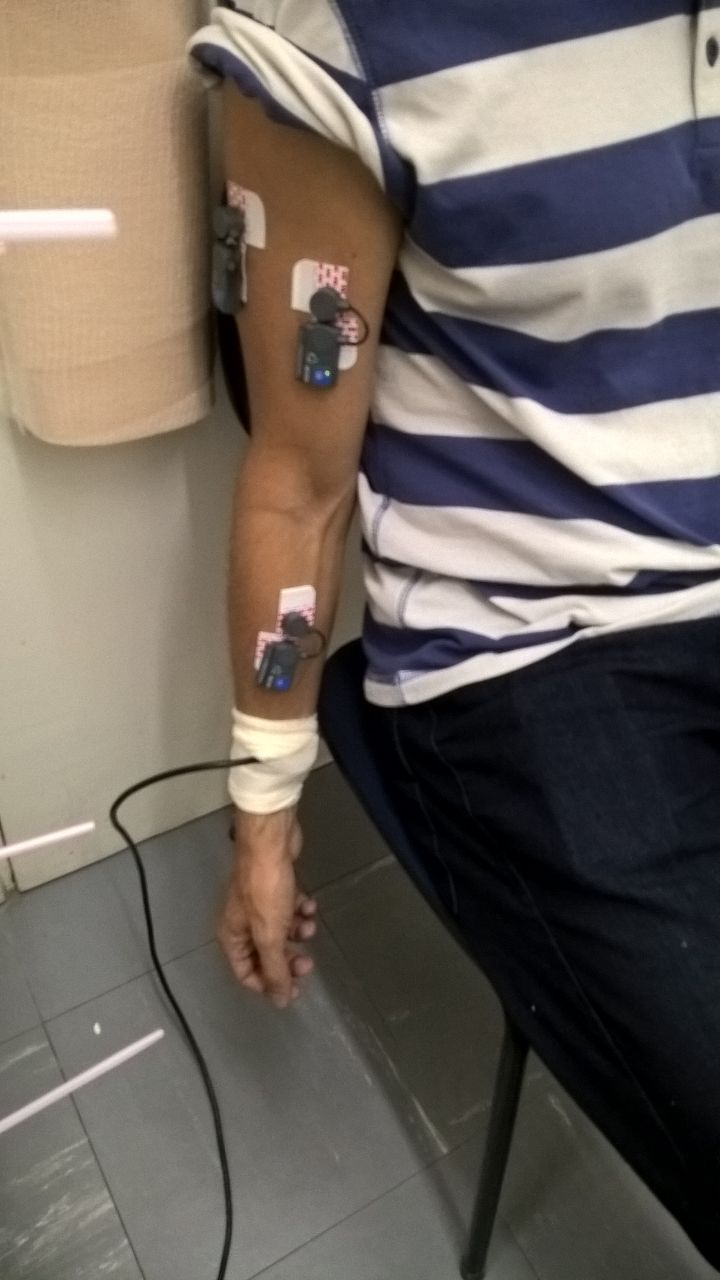
\includegraphics[scale=0.32]{Images/Experiment_Image.jpg}
      \caption{Experimental setup on a test subject}
      \label{Experimental Setup}
   \end{figure}

The subject sat on a chair, with the knees flexed at \(90^{\circ}\), the back perpendicular to the ground with the scapulas pressed against the wall. The back of the arm was leaning against a rubber support that was attached to the wall. This setup guaranteed that the subject was comfortable enough to perform repeated elbow flexions and extensions while maintaining the upper arm steady. 

The test protocol had three parts: The first one consisted of an isometric force test to obtain the Maximum Voluntary Contraction (MVC). The elbow of subject was kept in a fixed position at \(90^{\circ}\) and he/she was asked to apply the maximal possible force to flex the elbow. The subject was given a three minute interval before the next set.


In the second part, the subject was asked to perform five consecutive elbow flexion and extension movements from  \(50^{\circ}\) to \(140^{\circ}\) with a frequency of 0.5Hz. To help the subject reach the correct target angles a template was attached to the wall parallel to the subject, to provide visual guidance. To achieve the desired movement speed a metronome was set at the speed of 60 bpm so that the subject could synchronize the movements with the sound of the metronome.    

   The subject was given a minute of rest before the third part of the experiments. In this part the subject was asked to make an elbow flexion for 1s, then hold his forearm at \(140^{\circ}\) for 1 second, then a 1 second extension movement and then hold his forearm at \(50^{\circ}\) for another second. This movement should be repeated five times. Another one minute resting time was given to the subject.
Both of the continuous and interval tests were repeated with 1.5kg and 3kg extra weight placed at the subject's hand.

No subjects reported fatigue during the experiment.

The test was repeated in a different day, on all test subjects to further analyze the repeatability of the model proposed in this work.

All the data from the tests were transferred to Matlab\textsuperscript{\textregistered} for further analysis and processing.



\subsubsection{Experimental Data Processing}

The EMG data were processed as follows. Further explanations can be found on the literature \cite{Rose20161112}\cite{hayashibe:lirmm-00429594}
\begin{enumerate}
\item high-pass filtering of the EMG data, using a 2nd order Butterworth filter, with a cutoff frequency of 30 Hz, thus removing movement artifact.
\item Wave rectification
\item Second Order Butterworth Filter, with 1Hz cutoff frequency.
\item normalization with the peak of Maximum Voluntary Contraction (MVC)
\end{enumerate}

This way, the EMG is smoothed and presented as a percentage of the subject MVC instead of Volts.

A low-pass, 5 Hz cutoff frequency, second-order Butterworth filter is applied to the angular data to remove errors and other undesired signals.

Since the position tracking data was sampled at 100 Hz while the EMG data was sampled at 1KHz, all the position tracking data was resampled to 1000 Hz, an antialiasing finite impulse response (FIR) lowpass filter was applied and the delay introduced by the filter was compensated.

Figure \ref{Angle and EMG} shows an example of the recorded elbow angle and processed sEMG for the continuous movement with no extra weight.


\begin{figure}[thpb]
      \centering
      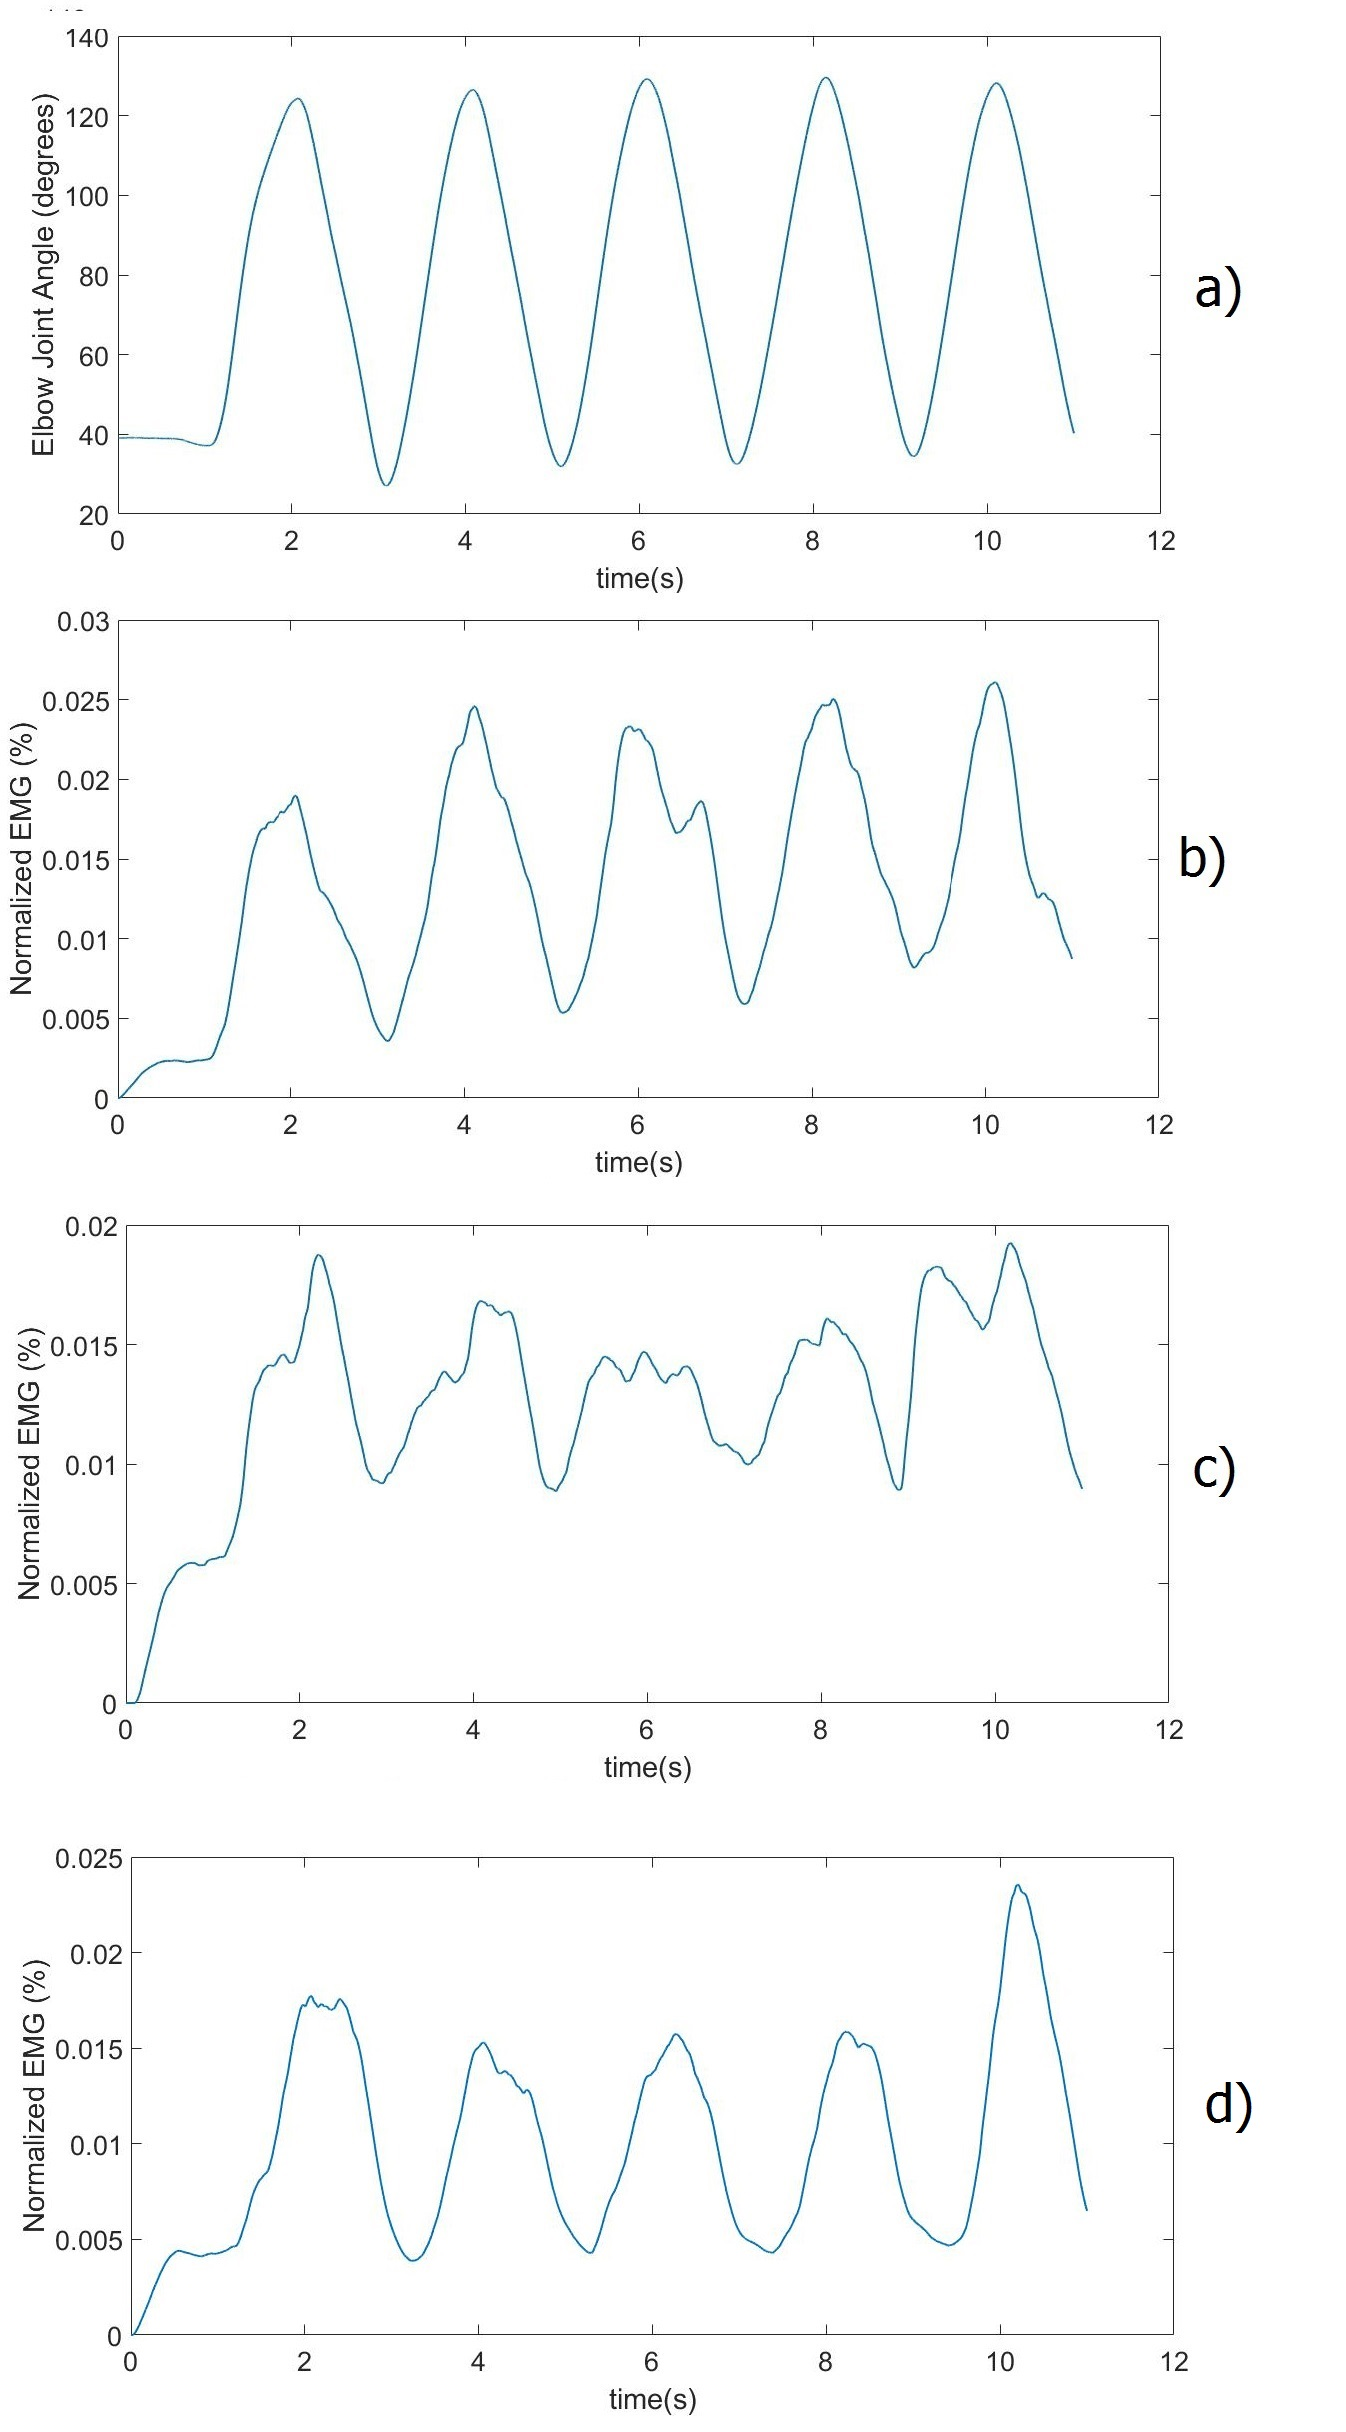
\includegraphics[height = 0.8\textheight]{Images/Angle_and_EMGs.jpg}
      \caption{a) Joint angle for the continuous movement with no extra weight, recorded with the IMU; sEMG values for the b) biceps brachii, c) triceps brachii and d) brachioradialis for the continuous movement with no extra weight.}
      \label{Angle and EMG}
   \end{figure}


\section{Linear System Modeling}

\begin{figure}[thpb]
      \centering
      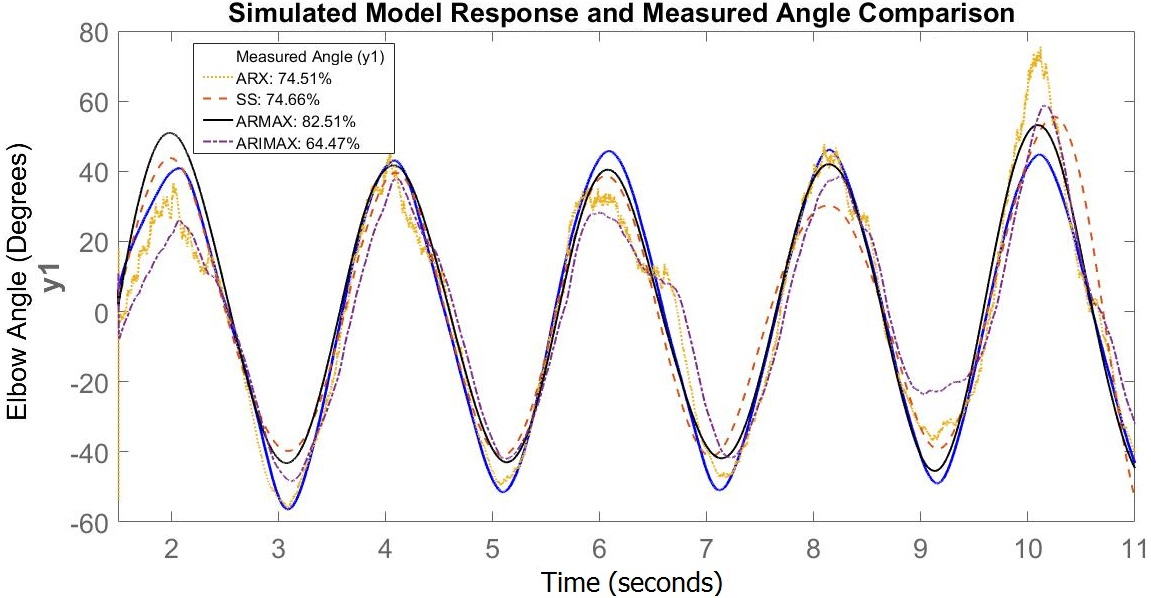
\includegraphics[scale=0.5]{Images/Models_comparison_5.jpg}
      \caption{Estimated elbow angle using the models responses compared to the elbow angle measured with the IMU. The estimated models were ARX, State Space, ARMAX and ARIMAX.}
      \label{Models Comparison}
   \end{figure}

It was assumed that the arm has the same model with different inertia parameters for the different weights attached to the arm of the subject arm. Considering a simple model of the elbow (arm with only 1 degree of freedom): 

\begin{equation}\label{eq:simpleModel}
T = (J + M\cdot L^2)\cdot \ddot{\theta}  + B \cdot \dot{\theta}  + (m\cdot l + M \cdot L) \cdot g \cdot cos(\theta)
\end{equation}


Where T is the elbow joint torque, J is the forearm inertia, B is the damping factor of the joint, m is the forearm mass, M is the dumbbell's mass, g is the gravity force and \(\theta\) is the joint angle. From this simple model it is easy to infer that, by changing the dumbbell's mass, the arm model parameters also change.

Four different modeling techniques were applied to determine which one best estimated the model that provides the elbow angle as an output taking the three EMG signals as inputs. These modeling techniques were: Auto-Regressive with Exogenous Input (ARX), Auto-Regressive Moving-Average with Exogenous Input (ARMAX), Auto-Regressive Integrated Moving-Average with Exogenous Input (ARIMAX) and State Space (SS).

To determine the best modeling technique, 10 models of each type were created with random parameter orders. Their estimation of the elbow joint angle was compared with each other. The model with the best fit value was chosen.  

With the model estimation technique chosen, it is necessary to determine the order of its parameters. To determine the chosen model order, 400 random combinations were tested for each data set with order values going from 0 to 10. The order chosen was the one that gave the best fit (see eq. \ref{eq:NRMSE}) between the estimated value and the one measured by the experiment. The coefficients of the models were estimated using time-domain data in Matlab\textsuperscript{\textregistered} (The Mathworks Inc, USA), minimizing a quadratic prediction error criterion.

To determine the best fit the normalized Root-mean-square error (NRMSE)  was used:
\begin{equation}
\label{eq:NRMSE}
NRMSE = 100*\left(1- \frac{||y-\hat{y}||}{||y-mean(y)||}\right)
\end{equation}

Where $y$ is the reference signal and $\hat{y}$ is the signal being evaluated.

\subsection{Results}

Figure \ref{Models Comparison} compares the different models with measured elbow angle and shows the fitness value for each data set.
The ARMAX model has the highest fitness value. For this reason it was the chosen model for the consequent estimations.

The ARMAX model has the following form:

\begin{equation}
A(q)y(t) = B(q)u(t-n_k)+C(q)e(t)
\end{equation}


Where y(t) is the output at time t, angle of the elbow joint, in this case; u(t) are the inputs, being the processed sEMG values from biceps brachii, brachioradialis and triceps brachii; e(t) is the white-noise disturbance; \(n_k\)  is the delay for each input; q is the delay operator; A, B and C are the model coefficients, defined by:

\begin{equation}
A(q) = 1 + a_1q^{-1}+\dots+a_{n_a}q^{-n_a}
\end{equation}
\begin{equation}
B(q) = 1 + b_1q^{-1}+\dots+b_{n_b}q^{-n_b+1}
\end{equation}
\begin{equation}
C(q) = 1 + c_1q^{-1}+\dots+c_{n_c}q^{-n_c}
\end{equation}


Where \(n_a\) is the system's number of poles; \(n_b\) is the number of zeroes plus one; \(n_c\) is the number of C coefficients.

The coefficient orders were calculated and can be found in table \ref{ta:order}.

\begin{table}[h]
\caption{Model parameters orders for each subject.}
\label{table_example}
\begin{center}
\begin{tabular}{|c|c|c|c|c|}
\hline
 & \(n_a\) & \(n_b\) & \(n_c\) & \(n_k\)\\
\hline \hline
Subject 1 & 1 & 1, 1, 4 & 1 & 8, 7, 0\\
\hline
Subject 2 & 1 & 1, 1, 4 & 1 & 8, 7, 0\\
\hline
Subject 3 & 1 & 1, 1, 4 & 1 & 8, 7, 0\\
\hline
Subject 4 & 1 & 1, 1, 4 & 1 & 8, 7, 0\\
\hline
Subject 5 & 1 & 1, 1, 4 & 1 & 8, 7, 0\\
\hline
Subject 6 & 1 & 1, 1, 4 &1 & 8, 7, 0\\
\hline
Subject 7 & 5 & 10, 3, 2 & 6 & 5, 3, 4\\
\hline
\end{tabular}
\end{center}

\label{ta:order}
\end{table}

\begin{figure}[thpb]
      \centering
      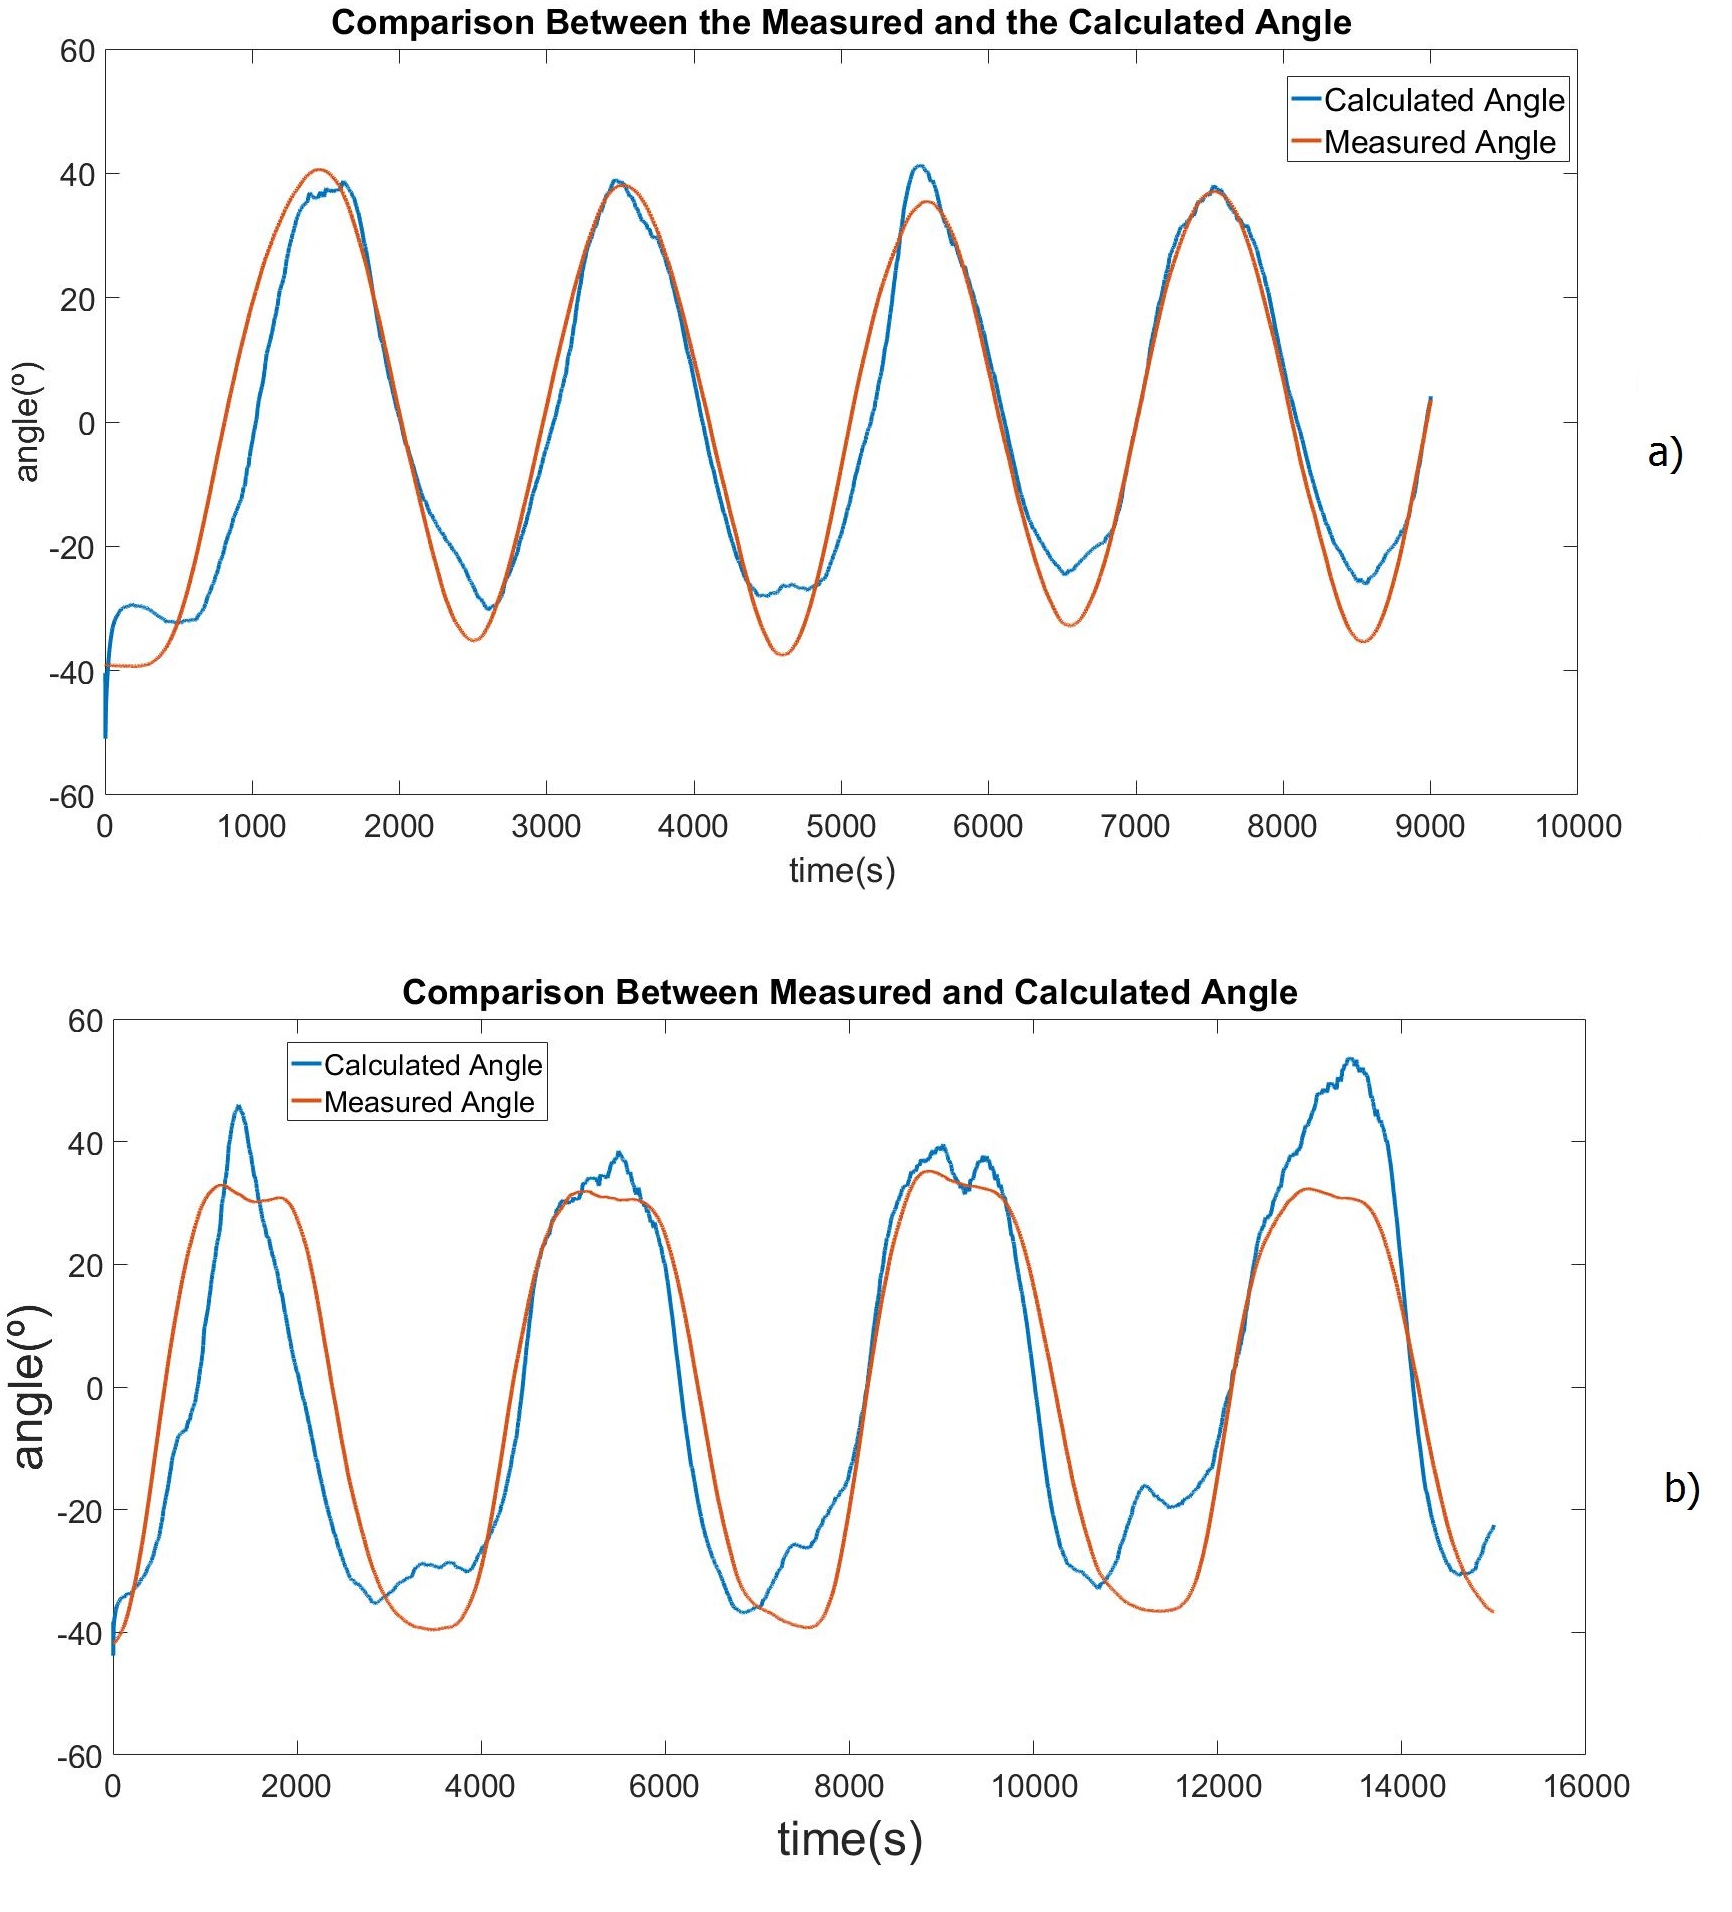
\includegraphics[scale=0.3]{Images/3kg.jpg}
      \caption{Comparison between the measured angle of the elbow joint and the angle calculated through the use of the estimated model, for subject 5. a) shows the comparison for the continuous movement and b) the comparison for the discrete movement}
      \label{Angle Comparison}
   \end{figure}

Using the values from table \ref{ta:order} as the ARMAX model orders, it was possible to calculate the model for elbow joint angle using the three sEMG measurements and compare it to the experimentally measured values. As an example, figure \ref{Angle Comparison} shows a comparison between the calculated and measured angle, for continuous and intermittent movement, for subject 5.

With the ARMAX model calculated for the test subjects, we aimed at validating the model. Using the same model order and parameters previously calculated we estimated the response of the system using a second batch of recorded data. An example of the result of this process can be seen in figure \ref{Validation Procedure}, where the model calculated for the subject number 3 was used to estimate the elbow joint angle using the input data acquired from the second day of testing.

\begin{figure}[thpb]
      \centering
      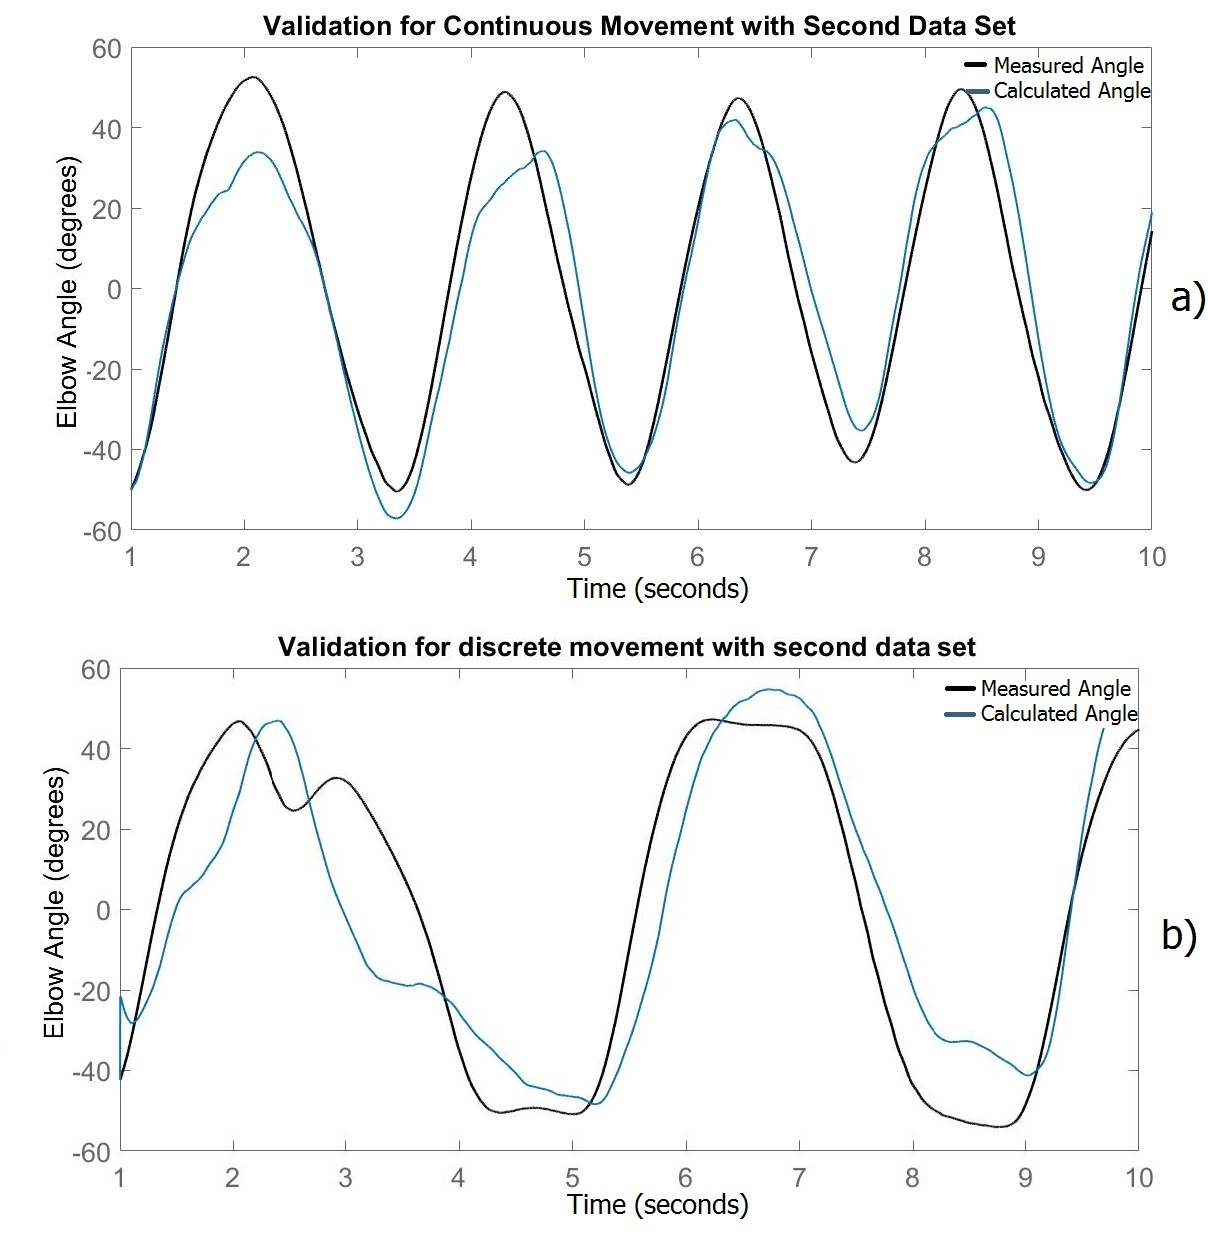
\includegraphics[scale=0.5]{Images/validation.jpg}
      \caption{Validation procedure to determine if the calculated model can be applied to the same test subject for tests made in different days. a) shows the comparison for the continuous movement and b) the comparison for the discrete movement}
      \label{Validation Procedure}
   \end{figure}

To better determine the accuracy of the model, two performance parameters were used: The correlation and the root-mean-square error (RMSE)  between the estimated and the measured elbow joint angles. Table \ref{ta:corr} shows the accuracy evaluation parameters for every test subject and every test set.


\begin{table}[h]
\caption{Correlation factor and Root-mean-square error for the estimated and measured angle values}
\label{table_example}
\begin{center}
\resizebox{\columnwidth}{!}{%
\begin{tabular}{|c c|c c|c c|c c|c c|}
\hline
\multicolumn{2}{|c|}{} & \multicolumn{4}{c|}{Calibration Test} & \multicolumn{4}{c|}{Validation Test} \\
\hline
\multicolumn{2}{|c|}{} & \multicolumn{2}{c|}{Continuous} & \multicolumn{2}{c|}{Intermittent} & \multicolumn{2}{c|}{Continuous} & \multicolumn{2}{c|}{Intermittent} \\
\hline
\multicolumn{2}{|c|}{} & Correlation & RMSE & Correlation & RMSE & Correlation & RMSE & Correlation & RMSE\\
\hline \hline

& 0 kg &0.8914 &15.61 &0.8218 &20.65 & 0.8966 & 29.85 & 0.9107 & 18.44 \\
Subject 1 & 1.5 kg &0.7761 &16.66 &0.8251 & 15.19 &0.825 &18.48 & 0.47 & 34.9\\
& 3 kg &0.9497 &13.82 &0.9011 &16.85 & 0.6123 & 29.13 & 0.8488 & 18.85\\
\hline

& 0 kg &0.9285 &11.29 &0.9659 &9.51 & 0.8249 & 19.28 & 0.941 & 20.43\\
Subject 2 & 1.5 kg &0.8011 &26.33 &0.897 & 16.59 & 0.8735 & 17.48 & 0.8935 & 22\\
& 3 kg &0.9314 &11.85 &0.9368 &13.7& 0.8666 & 16.32 & 0.8906 & 18.61\\
\hline

& 0 kg &0.8682 &19.47 &0.9123 &16.29 & 0.9033 & 18.04 & 0.8572 & 20.17\\
Subject 3 & 1.5 kg &0.9383 &16.61 & 0.9413& 12.42 & 0.922 & 16.045 & 0.9109 & 16.61\\
& 3 kg &0.9341 &13.66 &0.9602 &10.43& 0.9852 & 16.4 & 0.9048 & 17.16\\
\hline

& 0 kg &0.8806 &19.63 &0.88 &21.56 & 0.752 & 29.62 & 0.8931 & 21.87\\
Subject 4 & 1.5 kg &0.9408 &16.052 &0.9199 &17.95 & 0.3377 & 66.23 & 0.7704 & 39.44\\
& 3 kg &0.9608 &17.628 &0.862 &21.86 & 0.6104 & 139.73 & 0.7643 & 53.31\\
\hline

& 0 kg &0.8974 &18.805 &0.873 &24.68 & 0.9407 & 44.398 & 0.9192 & 16.322\\
Subject 5 & 1.5 kg &0.9233 &27.954 &0.823 &17.31 & 0.8801 & 15.427 & 0.8784 & 16.912\\
& 3 kg & 0.9621&7.286 &0.9239 &10.89& 0.8652 & 21.81 & 0.8445 & 24.316\\
\hline

& 0 kg &0.9256 &14.311 &0.9029 &20.76 & 0.8793 & 34.11 & 0.9258 & 53.08\\
Subject 6 & 1.5 kg &0.8184 &19.37 &0.828 &19.93 & 0.7782 & 21.96 & 0.9317 & 26.05\\
& 3 kg & 0.8323 & 19.13 &0.9169 &16.3 & 0.7722 & 102.16 & 0.8043 & 31.88\\
\hline

& 0 kg &0.9147 &18.515 &0.9057 &15.48 & 0.8063 & 19.335 & 0.9 & 15.815\\
Subject 7 & 1.5 kg &0.9066 & 12.424&0.9411 & 11.85 &0.8728 & 17.035 & 0.887 & 18.509\\
& 3 kg &0.9194 &12.857 &0.949 &12.6 & 0.7825 & 18.16 & 0.931 & 15.12\\
\hline

\end{tabular}%
}
\end{center}

\label{ta:corr}
\end{table}

\subsection{Non-Linear System Modeling}

\subsection{Results}

\subsection{Discussion and Conclusions}

This chapter proposed a method for determining the elbow joint angle based on the measurement of the sEMG of biceps brachii, triceps brachii and brachioradialis from 7 test subjects. The arm model was estimated using the data collected from the experiment and a system identification method, more specifically, ARMAX. Using the acquired sEMG data as input to the estimated model, it was possible to obtain an estimation of the elbow angle. Using the data from the IMU (real angle value) it was possible to validate the estimation based on sEMG.

The experimental data showed that it is possible to use only the EMG data to estimate a correlation between joint angle and sEMG values. Even though estimating one model for continuous movement and another one for discrete movement gives higher precision, it is possible to calculate a single model for both movements.

As stated before, by lifting different weights the model parameters are altered.
For the same test subject the A(q) and C(q) parameters (see eq. 3) maintained values with less than 1\% difference from one another, while the B(q) values assumed a greater range of values.

Even for different subjects, the estimated A(q) and C(q) parameters also had a difference of less than 1\% from one another.

From the seven subjects, six of them could be estimated by an ARMAX model with the same parameters order. The test subject with different order parameters was the one that presented the worst readings of the brachioradialis muscle EMG. Because of that, a lot of noise is introduced, requiring a higher order system to overcome the modeling errors. The brachioradialis is the most difficult muscle to read the sEMG signals compared to the biceps brachii and the triceps brachii. This difficulty is due to the muscle short length causing the electrodes to stay close to the tendon, which induces  reading errors. Not coincidentally, this test subject was the one with smaller stature.

The repeatability of the model was successful for the cases studied in this work, even though it is possible to note that the model is not as precise as it was for the calibration procedure.

In future works it will be studied if it is possible to define one single estimated model for each subject, independent of the weight being lifted, or even one global model that is capable of estimating joint angles for a big range of individuals. The calculated models will be used for the control of an EMG-driven upper limb exoskeleton.